%************************************************
\chapter{Modelling the Dynamic}
\label{chapter:modelling_the_dynamic}
%************************************************

\begin{figure}[bth]
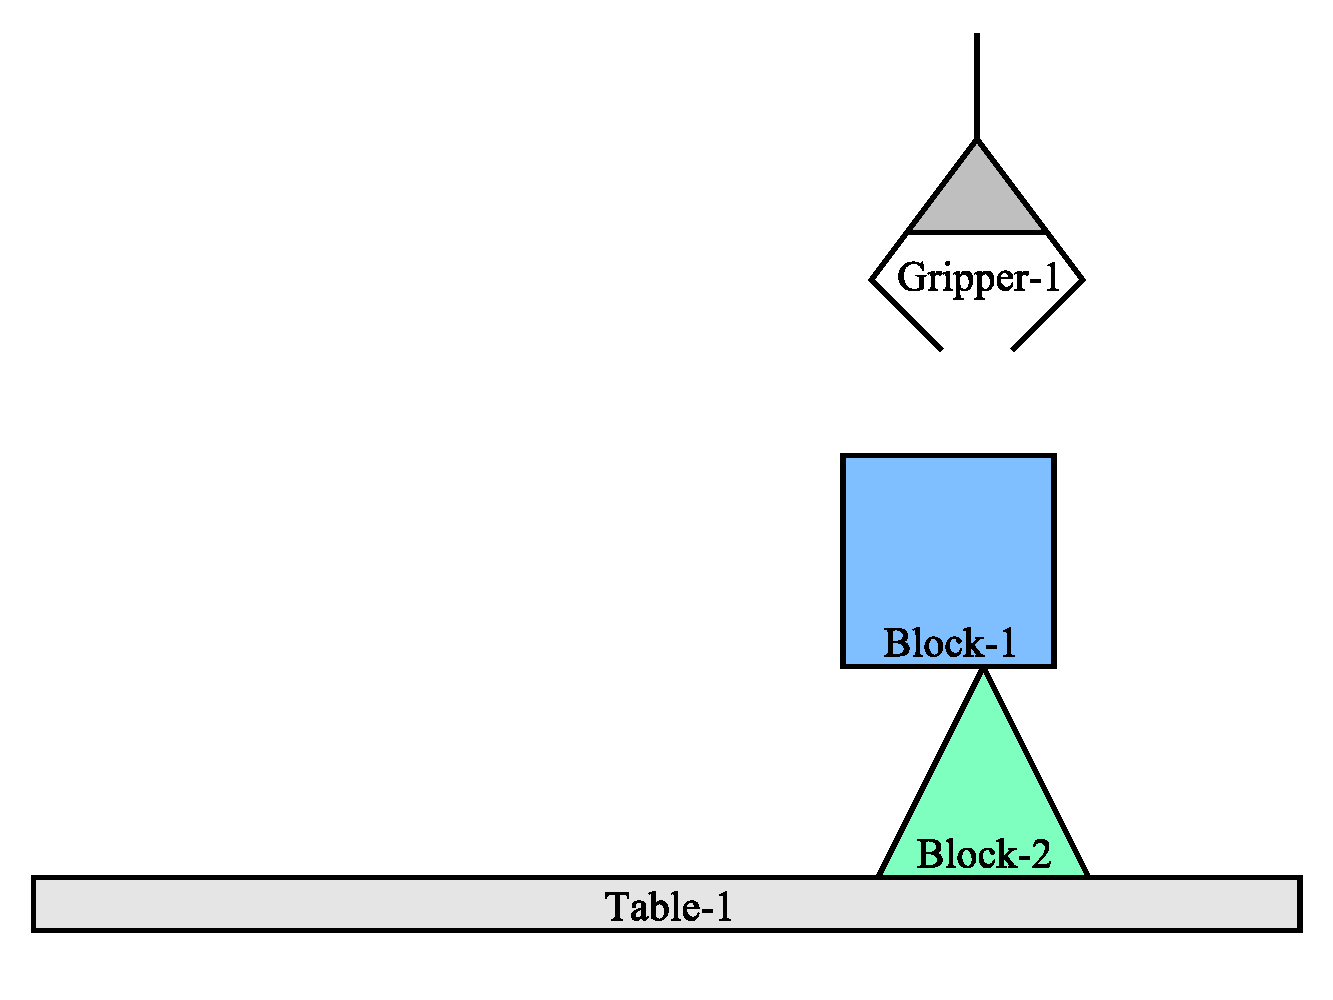
\includegraphics[width=10cm]{gfx/blocks_world_example_failure} \\ \medskip
\caption{A failure to stack two blocks.}
\label{figure:example_of_failure}
\end{figure}

My thesis is SALS, a computational simulation of a model of learning
in multiple reflective layers.  I begin my explanation with a
description of the example situation pictured in
\autoref{figure:example_of_failure}:
\begin{quote}
There is a table.  Some blocks are on the table.  The blocks are of
different shapes and colors.  One of the blocks is a green triangle.
Another block is a blue square.  A gripper can move around, picking up
and putting down blocks.  Plans are made for the gripper to arrange
the blocks into different configurations.  Plans are followed that
sometimes result in a failure.  For example, putting the square on top
of the triangle fails to stack the two blocks because the square falls
off of the triangle.  A single failure is a learning opportunity.  A
better model of the world can be learned through each failure.
\end{quote}
This is a common type of situation for current learning algorithms,
updating models of the world when experiences fail to match
expectations.  What I show in this thesis is that better models of
planning strategies can also be learned from these same failures.
Learning different planning strategies for different situations is a
reflective form of thinking.  Thus, my thesis is SALS, which provides
a working example of turning a single failure into failures at
multiple reflective layers, demonstrating multiple learning
opportunities from a single failure.

I begin with a non-technical description of the model in plain
English.  At the end of \autoref{part:the_model}, I explain the
modelling assumptions that I make in transitioning to the mathematical
notation of \autoref{part:simulating_the_model}.  Using this notation,
I explain how this model can be used to reduce the complexity of
search algorithms.  In \autoref{part:the_implementation}, I give an
explanation of how this simulation is automated on a concurrent
computer, the thesis implementation, SALS, the substrate for
accountable layered systems.  In conclusion, in
\autoref{part:conclusion}, I discuss promising directions for future
research in not only AI but also the other cognitive sciences.

\section{About the Description}

In this dissertation I focus on a description of thinking that
reflectively learns to accomplish goals.  I begin with the paradoxical
task of describing reality, that which actually exists.  My model of
reflective thinking grows quickly within this initial foundational
conception of reality, which, as it begins reflectively, leads
necessarily but naturally to the goals of this dissertation.  This
first part of the dissertation gives a non-technical, but complete,
understanding of my reflective model of mind.

I will not attempt to give a complete representation for a general
problem domain nor a complete description of a general problem solver.
My work here leaves the unmodellable aspects of reality as known to be
just that.  Thinking uses models as useful tools with the clear
understanding that these models are not fundamentally real.  Further,
and critically important for the advancement of the field of AI, when
describing reflective thinking, it is imperative to have an explicit
awareness of thinking being limited to manipulating the artificial.  I
will therefore refer to an AI model as simply an ``AI'' with the
shared understanding that I am referring to a model.

Non-reflective AI models learn by correcting one immediate cause of a
failure; however, given a layered model, I describe new opportunities
for considering one failure to also be failures in the reflective
layers ``above'' and ``below'' the original failure, resulting in an
arbitrary number of reflective learning opportunities from a single
failure.

In \autoref{part:the_implementation}, I will describe an example of a
computational implementation of reflective thinking.  The
implementation is a layered cognitive architecture with three working
layers.  I will focus on a very simple physical block stacking problem
domain as a tool for explaining simply, through examples, the layered
classes of reflective learning.  In describing the working model
implementation, I will maintain an awareness of the explicit
distinction between a model and reality.  I have categorized my focus
in this way only as an example of the computational description.

\section{Meaningful Description}

A meaningful description references reality.  Words and language have
meaning only in this way.  The further ability of words to also
reference other words allows the additional possibility of creating a
referential circularity in language.  An illusion of a primitive
meaning is possible in such a cycle because all of the words have a
referent; however, because all references within such a closed cycle
appear to be exclusively kept within language and do not seem any
longer to refer to anything real, there is a danger of there being no
meaning other than circularity to such a purely artificial construct.
Again, symbols are tools for modelling and are useful only if the
tautology inherent in the circularity is not forgotten as being
artificial.  Thus, I avoid strictly presenting such illusions of
meaning as primitive in this dissertation.  To allow for meaningful
descriptions, I will first outline my conception of reality, to which
my description ultimately must refer.  A description of reflective
thinking referring to an \emph{a~priori} concept that has not been
derived in terms of symbols allows for something to remain outside of
language as the real referent.  This last step avoids the creation of
a cyclical, self-referential tautology and prevents illusions from
becoming meaningful parts of the model.  In the next section I will
describe the necessary conception of reality to which my description
of reflective thinking will refer.

\section{Qualities of Duration}

\cite{bergson:1910}, in his seminal \underline{Time and Free Will},
discusses reality as heterogeneous qualities of Duration.  Qualities
of Duration will serve as my conception of reality for my description
of reflective thinking.  Qualities of Duration are the dynamic ongoing
activity, heterogeneous qualities that are neither distinct nor
separate.  There is a trick, a sort of slight of hand, required here
in describing Bergson's conception of the qualities of Duration
because these qualities exist independently of symbolization.  For
example, when I look at a tree, I may say that the tree has green
leaves and a brown trunk; the symbols, green and brown, refer to the
qualities of Duration, which I am really seeing.  When I focus
carefully on the reality of my situation, I see that the leaves and
trunk could be described by a greater combination of various greens,
yellows, grays, browns and reds.  Symbols limit perception to a
discrete sort of projective presupposition.  Therefore, as I introduce
more symbolic references in my increasingly limited description of
reality, a growing danger of losing focus on something real emerges,
creating a cycle of symbols seemingly referring exclusively to
symbols.  For example, the motivation to tangentially define more
clearly what I mean by the symbol green or brown by using more symbols
results in a circularity from which there is no exit, and therefore, a
false dilemma from which I will never again be able to see or talk
about any real tree as the referent.  In order to avoid the danger of
purely cyclic symbolic references in my model, I will continue to
relate the parts of my model to real reflective thinking, which exists
as qualities of Duration.

\section{Consciousness, Awareness, and Experience}

There are many terms that are used in the literature when referring to
the concept of reality.  Each of these terms has a different
associated collection of necessary absurdities.  For example, the term
consciousness begs the question \emph{of what} one is conscious.
There is an implied subject and object relationship when using this
transitive term, which is not meant when the term is used as an
isolated absolute reference to reality.  The terms awareness and
experience are used similarly and have the same necessary absurdities
as the term consciousness when they are considered as absolutely
singular references to reality.  Each of these terms has different
meaningful uses when they are not used in this absolutely singular
sense.  For example, in this dissertation an awareness of the
potential confusions these terms introduce when they are used
singularly in abstract isolation as reference to reality will be
maintained.  Thus, I will not argue that these conceptions of reality
are incorrect, but in order to avoid confusion, I will never use these
terms in their abstracted sense.  Instead, I will conflate all of
these uses of these terms as all being the same as my conception of
reality, the ongoing activity that my model accepts, symbolizes, and
thinks about as given.

Because my model of mind is a an absolute reference to reality, which
is everything that exists, it actually makes very few modelling
assumptions.  Because my model has been previously mistaken for the
philosophy of ``subjective idealism'', I have included a description
of the important difference between my model and this problematic
philosophy; I explain this critical difference in
\autoref{section:the_mistake_of_subjective_idealism}.

\section{Actual Reflection}

The qualities of Duration are the given dynamic ongoing activity.
These qualities are the inseparable actions that are currently
available to reflection.  Reflection is the ability to symbolize this
ongoing activity.  For example, the activity of perceiving a table can
be symbolized as ``table''.  Similarly, the activity of walking, can
be symbolized as ``walking''.  Note that my model of reflective
thinking assumes that there is ongoing activity before any symbols
exist for the actions of thinking to manipulate.  Thinking is an
auxiliary activity that manipulates artificial symbolic constructions
that refer to the primary ongoing activity of existence.  Thus, the
activity of perceiving a table requires neither that this activity be
reflectively symbolized nor that a secondary thinking activity
manipulates the resulting symbols.  I will use the phrase \emph{actual
  reflection} to refer to the activity of symbolizing ongoing
activity.

\section{Order of Space}

Qualities of Duration may be symbolized in a homogeneous medium
without quality.  Bergson calls this medium Space, allowing symbolic
references to qualities of Duration to be related.  Of major
importance is the fact that one does not derive the other, but quality
and order coexist with neither Duration being a derivative of Space
nor Space containing the fundamental qualities of Duration.
Obviously, Bergson has gone through painstaking efforts to leave room
in his description for reality as some independent, non-contingent
quality not derived from either Space or Duration.  He makes the
necessary concession that a description of something real is only
meaningful in that it leaves room for reality to exist independently
of its own symbolization.  This work is meant to be similarly
respectful in the description of reflectively learning to accomplish
goals.

\section{The Artificiality of Duration and Space}
\label{section:the_artificiality_of_duration_and_space}

Duration and Space are the fundamental duality that forms the basis of
my model of reality.  Thus this duality exists pre-reflectively, prior
to symbols being created from the qualities of Duration and prior to
these symbolic references being related in Space.  Note the
fundamental contradiction of intentionally describing reality only in
artificial terms.  For example, if Space has no quality and is not
itself composed of qualities of Duration, to what is the symbol
``Space'' referring?  Symbol ``Space'' refers only to the logical
potential for an absence of quality, the potential for itself as not
really existing; thus, it is the logical necessity of the negative
implication of positive existence, to which no real alternative can be
assigned.  Again, my model will explicitly maintain an awareness of
this implicit, fundamental and irresolvable contradiction.  Thus, my
description will appear to begin of something in the middle, the
\emph{in medias res} of an underived time and space, maintaining an
explicit awareness that descriptions are only tools for reflection.
Duration and Space are not placeholders for reality; they are useful,
intermediate fictions that I use here to artificially and statically
describe the dynamic ongoing reality, the activity of being, that
which is not artificial.

\section{Spatial Reflection}

The qualities of Duration are the real activity of being in the
present, actively dynamic and ongoing.  Symbols are artificial static
references to the dynamic present.  Actions are the qualities of
Duration, whether or not they are symbolized.  There is a fundamental
distinction here between the dynamic and the static.  The ongoing
dynamic is actual, while the arrested static is artificial.  In this
way, spatial relationships between symbols can actually exist in
reality as an actively maintained artificial construction.  The
qualities of the ongoing activities that hold symbols in a specific
Spatial arrangement can be symbolically reified.  I will refer to the
activity of symbolizing the qualities of a Spatial arrangement of
symbols as \emph{Spatial reflection} or \emph{reification}.  Spatial
reflection is a form of actual reflection.

\section{The Physical Layer}

My model includes three layers of ongoing dynamic activity.  I will
use the phrase \emph{physical layer} to refer to the pre-reflective
layer of activities that exists necessarily prior to any subsequent
reflective thinking layers.  The physical layer is the only
pre-reflective layer of activity in my model.  Therefore, a clear line
is drawn between the physical layer and those activities that
symbolize and Spatially arrange symbols.  Thus, they are not included
in what I will refer to as physical activity.  Note that in most AI
models, there is a distinction between the mind and the body or the
environment.  In my model, \emph{all} activities that exist are part
of the mind.  The real mental activities that I am referring to in my
model are not an object that is viewed subjectively.  Critical to an
understanding of the goals of objective science is that the creation
of object and subject distinctions is part of the activities of the
mind; because this understanding is so critical to an advancement of
scientific understanding, I will clarify the mental derivation of
objective science in \autoref{chapter:science}.  Because the creation
of object and subject relationships is a relatively advanced mental
activity and not key to my thesis, I will discuss this as future
research in \autoref{chapter:future}, which would be a promising place
to extend my model to include ideas like physical bodies and other
subjective and objective environmental perspectives.

\section{Orders of Reflective Layers}

In addition to the pre-reflective physical layer of activity, my model
includes two additional layers of reflective thinking activity that
use two different classes of causal models in order to accomplish two
different classes of goals.  I will use the phrase \emph{first-order
  reflective layer} to refer to the reflective layer of thinking that
creates symbols and Spatial arrangements that refer to physical
activities.  I will refer to reflectively symbolizing physical
activities as \emph{physical reflection}.  Physical reflection is a
form of actual reflection and is one of the primary reflective
thinking activities; remember that physical activities are
pre-reflective, so physical reflection is not itself a physical
activity.

Obviously, the first-order reflective layer cannot create symbols or
Spatial arrangements that refer to its own activities, with one
exception: Spatial reflection.  The first-order reflective layer has
the \emph{a~priori} ability to maintain its own actively reified
Spatial relationships as existing between symbols that refer to
physical activities.  The lack of the ability for the first-order
reflective layer to refer to its own symbolically creative or
Spatially manipulative activities clarifies my model by keeping clear
distinctions between each class of causal knowledge in each subsequent
reflective layer of thinking.  Before describing distinctions between
classes of causal models, I will spend the next few sections
describing the composition of temporal transitions and causal
hypotheses.

Reflection over the activity of the first-order reflective layer
necessarily creates a second layer of reflection and thinking.  Thus,
clearly deriving and describing this second layer of reflective
thinking additionally necessitates an implicit and arbitrary number of
layers.  This condition is the focus of this dissertation.
\cite{minsky:2006} describes a six-layer reflective model of thinking
about thinking.  The first three layers of my model and
implementation, including these two layers of reflective thinking, can
be compared to the first four layers of Minsky's model.  There are
many close parallels between my model and Minsky's model, and I will
describe these as implementation parallels in
\autoref{part:the_implementation}.

\section{Intensities of Qualities}
\label{section:intensities_of_qualities}

\cite{bergson:1910} makes a key distinction between comparisons of
``extensive'' quantities and comparisons of ``intensive'' quantities.
Extensive quantities are Spatial comparisons.  Extensive quantities
are between two symbolic references that share a containment
relationship in terms of their referents: one symbolic referent is
inclusively contained by another symbolic referent in Space.  For
example, one body may be said to be larger than another in terms of
its Spatial extent.  Intensive quantities are more subtle and an
example is in terms of pain, which can be said to be more or less
intense.  Intensive quantities are similar to neither numerically nor
Spatially extensive containment relationships but, instead, refer to
different fundamental qualities of Duration.  For example, a pain that
has no intensity is not a pain at all; a pain that has a mild
intensity may be equivalently referred to as an irritation or an itch;
a pain of high intensity may be equivalently referred to as a sharp
pain or a throbbing pain.  The point is that these intensities of
quality are actually very different from extensive quantities in that
they are not greater than or less than one another in the sense of a
containment relationship.  For example, a very intense pain, such as a
shooting pain or a throbbing pain, does not in any sense contain a
lesser mild pain, such as an irritation or an itch.  This same pattern
exists with detailed descriptions of other qualities that are often
thought of as having comparable intensities: heat and cold; light;
pressure; sound; pitch; aesthetic feelings, such as grace and beauty
in music, poetry and art; emotions, such as rage and fear; moral
feelings, such as pity; affective sensations, including pleasure, pain
and disgust.  Each of these examples points out that the apparent
relationships of greater than or less than with respect to intensity
are actually artificial Spatial arrangements of different fundamental
qualities of Duration.

\section{Number}
\label{section:number}

\cite{bergson:1910} shows the derivation of all numerical
representations as requiring an accompanying extension in Space.  For
example, in referring to the individual sheep in a flock of sheep, he
explains counting:

% pg. 75-77
\begin{quote}
Number may be defined in general as a collection of units, or,
speaking more exactly, as the synthesis of the one and the
many\ldots

No doubt we can count the sheep in a flock and say that there are
fifty, although they are all different from one another and are easily
recognized by the shepherd: but the reason is that we agree in that
case to neglect their individual differences and to take into account
only what they have in common.  On the other hand, as soon as we fix
our attention on the particular features of objects or individuals, we
can of course make an enumeration of them, but not a total\ldots

Hence we may conclude that the idea of number implies the simple
intuition of a multiplicity of parts or units, which are absolutely
alike.

And yet they must be somehow distinct from one another, since
otherwise they would merge into a single unit.  Let us assume that all
the sheep in the flock are identical; they differ at least by the
position which they occupy in space, otherwise they would not form a
flock.
\end{quote}

The last point here illustrates the idea that numbers are always
derived from symbols situated in Space.  Therefore, a model for
thinking based directly on the symbols required cannot be more
complicated than a model based on a numerical representation.  A
number is, after all, the reified constructive result of an assumed
Spatial organization of symbolic references to reality, specific real
sheep.  The explicit implication is, therefore, that, in building an
AI that is capable of reflective thought, model building and the use
of numerical representations must be explicitly available for
inspection by the AI itself.  Here, I employ Occam's razor to simplify
the loop of reflective representation in order to ease building the
first proof-of-concept examples of AIs capable of reflective thinking.

\section{Time as Space}

Symbolic references can be ordered spatially.  These symbolic
relationships can be reified and treated symbolically by further
ordering spatial relationships.  Thus, Bergson explains time as a form
of Space:

% pg. 98
\begin{quote}
Now, if space is to be defined as the homogeneous, it seems that
inversely every homogeneous and unbounded medium will be space.  For,
homogeneity here consisting in the absence of every quality, it is
hard to see how two forms of the homogeneous could be distinguished
from one another.  Nevertheless it is generally agreed to regard time
as an unbounded medium, different from space but homogeneous like the
latter: the homogeneous is thus supposed to take two forms, according
as its contents co-exist or follow one another.  It is true that, when
we make time a homogeneous medium in which conscious states unfold
themselves, we take it to be given all at once, which amounts to
saying that we abstract it from duration.  This simple consideration
ought to warn us that we are thus unwittingly falling back upon space,
and really giving up time.
\end{quote}

Time exists only as an artificial creation, a derivative arrangement
of symbols in Space.  Understanding time to be artificial is important
because this allows the real heterogeneous qualities of Duration and a
real homogeneous unqualified Space to remain, respectfully, neither
distinct nor separate.  By prohibiting this separation, and, thereby,
their independent existences, I avoid defining the real qualities of
Duration in terms of artificial symbols, avoiding the creation of a
self-referential cycle, thus sidestepping the potential illusion of a
purely tautological meaning by being clear in our understanding of
time used intentionally as an artificial tool of thought.

In my model, symbols are put into an artificial Spatial arrangement
that I refer to as time.  The actions that create symbols and put
these symbols into Space are basic parts of my model of reflective
thinking.

\section{Temporal Reflection}

Spatial arrangements of symbols can be used to represent a past
through memory and subsequently project an analogous ``future'',
through imaginative action, thus constructing a derivative conception
of time.  The past and the future, therefore, remain artificial
constructions that are actively maintained as Spatial relationships in
the present.  I will refer to the reification of Spatial relationships
that order the past and the future as \emph{temporal reflection}.
Sequential time is created through temporal reflection.  Temporal
reflection is a form of Spatial reflection.  Like Spatial reflection,
temporal reflection is also a form of actual reflection, symbolizing
the active maintenance of a temporal Spatial relationship between
static symbolic references.

\section{Simultaneity and Transition}

Correlation requires two symbols to be related in Space.  As symbols
are correlated in the Space called time, these temporal correlations
are referred to as either simultaneities or transitions.
Simultaneities represent two symbols that are both actively symbolized
in Duration.  Transitions represent the change from the past to the
future.  Transitions can be extended in time in order to create
counterfactual temporal extensions, called inferences.  Inferences of
the past and the future can be created by matching and repeating these
transitions.  A transition implies the removal of one symbol and the
addition of another as a progression is made through a temporal
sequence.  If correlations are counted and compared in ratios, then
these are called probabilistic correlations, and the resulting
inference would be a probabilistic inference.

